\documentclass[hidelinks]{article}
\usepackage[english]{babel} 
\usepackage[utf8x]{inputenc}
%% Hyperlinks 
\usepackage{hyperref}
\hypersetup{
    colorlinks,
    linkcolor={red!50!black},
    citecolor={blue!50!black}, linktoc=all,
    urlcolor={blue!80!black}
}
%% Graphics
\usepackage{graphicx}
\usepackage{float}

\usepackage{enumerate}
% Math packages
\usepackage{amsmath}
\usepackage{mathtools}
\usepackage{amssymb}
\usepackage{mathpartir}

% Proof system
\usepackage{amsthm}
%\usepackage{xpatch}
\makeatletter

% paper margins
\usepackage[tmargin=1.5in,lmargin=1in,rmargin=1in,bmargin=2in]{geometry}
% citations
\usepackage{cite}
% Graphs
\usepackage{tikz}
\usetikzlibrary{quotes,angles}

% multiple colums
\usepackage{multicol}

% Custom commands
\newcommand*\vtick{\textsc{\char13}}
\def\righttriangle{
\scalebox{0.7}{
\begin{picture}(5,0)
\hspace{-0.2em}
\put(0,0){\line(1,0){10}}
\put(10,0){\line(-1,1){10}}
\put(0,0){\line(0,1){10}}
\end{picture}
}
}

\pagestyle{plain}

%Title page settings
\usepackage[affil-it]{authblk}

% Title of document
\title{\textbf{Foundations of Mathematics\\and the Foundational Crisis}}
% Author
\author{Kevin Kappelmann}
\affil{Chair for Logic and Verification,\\ Technical University of Munich}
\date{\today}

% Quotes with author
\usepackage{xparse}

\let\oldquote\quote
\let\endoldquote\endquote

\RenewDocumentEnvironment{quote}{o}
  {\oldquote}
  {\IfValueT{#1}{\par\nobreak
   \hfill--- #1}\endoldquote\addvspace{\smallskipamount}}

% Line breaks after paragraph
\usepackage[parfill]{parskip}
% double line spacing
%\linespread{1.5}
%------------------------------------------------------------------------------
\begin{document}
\pagenumbering{gobble}
\maketitle
\vfill
\hfill
\mbox{
\begin{minipage}{0.27\textwidth}
	\textit{Young man, seek no longer,\\
	for what I have found\\
	is the only everlasting verity,\\
	in that there is no certainty\\
	and by this no truth.}
\end{minipage}
}
\newgeometry{margin=1.5in}
\newpage
\section*{Preface}
%\vspace{-1.8em}
Although --- or maybe even because --- mathematics is probably the most well-conceived and exact science of mankind, it has not been free of scepticism and controversies. At its heart, mathematics deals with the discovery of unchangeable, everlasting truths. For this, we use rigorous proofs. But what is it that we call a proof?

One might define a proof as a coherent chain of logical arguments leading from a set of premises to a conclusion. This definition, however, raises many new questions. What deserves to be called coherent? When is an argument logical? Does everyone follow the same rules of logic? Which premises are there to begin with?

Some of the greatest mathematicians intensively debated some of these questions in the beginning of the 20th century, namely during the foundational crisis of mathematics. The sophisticated foundations of modern mathematics are the results of these debates and the rigorous work that went into them. Contemporary mathematicians are thus able to concentrate on extending mathematics rather than worrying about its foundations. 

However, due to the invention of the computer in the late 20th century, the certainty of mathematics has once again been questioned as a new field of proof theory has arisen. At the time, computer scientists and mathematicians began to develop proof assistants and automated theorem provers. The former are designed to verify proofs entered by humans, the latter act on a fully automatic basis.

Automated theorem provers in particular gave rise to new questions regarding mathematical proofs. Does a computer-generated proof have the same credibility as a proof written by a person? How can I persuade somebody that my proof is indeed valid? Does it suffice to understand every isolated step, or do I need to understand its holistic idea? Must it be accepted by many, a few, or even just one person? 

These new questions and controversies are subjects for debate in the seminar ``Formal Proof in Mathematics and Computer Science'' offered by the Chair for Logic and Verification at the Technical University of Munich in 2017. This paper shall start off the seminar by giving a brief overview of the foundations of mathematics with a focus on the foundational crisis in the 20th century. Interested readers are able to find further papers from the seminar at \url{https://www21.in.tum.de/teaching/proof21/SS17/}.
\newpage

\tableofcontents 
\newpage

\pagenumbering{arabic}
\section{Historical introduction and controversies}
While one might think that mathematics as a subject about absolute certainty ought to be free of controversies, history taught us otherwise. In fact, it has been subjected to fiery disputations since ancient Greece. Before diving into the most famous controversy in the history of mathematics, namely the \textit{foundational crisis} (in German \textit{Grundlagenkrise}), we want to give a brief historical overview focusing on the foundations and some of the most well-known controversies\footnote{We emphasise the smaller extent and impact of various mathematical disputations by using the word \textit{controversy} as opposed to \textit{crisis}.} of mathematics.

\subsection{Ancient mathematics}

The history of mathematics is coined by a series of abstractions.
Add two apples to three other apples, and you get five apples. Add two bananas to three other bananas, and you get five bananas. We abstract our results and infer: two plus three equals five. The concept of numbers might be the first mathematical abstraction in history. Consequently, arithmetic together with geometry were unsurprisingly the first developed branches of mathematics, due to their intuitive nature.

First evidence for more complex mathematics dates back to around 2400 BC\@. Egyptians and Babylonians used basic arithmetic and geometry for trading, taxation, building and construction, and land measurement. Nonetheless, by that time mathematics was just regarded as an applied tool to solve practical problems rather than an exact science. Heuristics, pictures and vague analogies justified the use of given formulas as opposed to rigorous proofs.

The idea of demonstrating conclusions using coherent arguments, and thereby the development of the notion of a proof, was one of the great achievements in ancient Greece.
Beginning with Thales in 600 BC, mathematics as a means of the exploration of everlasting truths began to rise. Again, to no surprise, proofs where focused on arithmetic and geometry; both which seemed to consist of unquestionable verities.

In 500 BC, the Pythagoreans did not only discover one of the most famous theorems in mathematics --- the Pythagorean theorem\righttriangle --- but to our larger interest experienced the first noteworthy mathematical controversy. They were in firm belief that all numbers were commensurable; that is for every pair of non-zero numbers $a$ and $b$, the ratio $\frac{a}{b}$ is a rational number. It allegedly was the work of Hippasus who dismissed this ideal by proving the existence of irrational numbers. Legend has it that Hippasus was sentenced to death by drowning for the discovery of this unbearable truth. What remains as a fact is that Pythagorean mathematics changed drastically after this discovery.

Meanwhile, the Greek philosopher Zeno of Elea devised four paradoxes, now commonly known as Zeno's paradoxes, which mainly deal with the illusion of motion. The first paradox, referred to as \textit{Achilles and the Tortoise}, can be recounted as follows:
\begin{quote}\label{zeno_paradox}
Achilles and the Tortoise want to conduct a race. As he clearly is the faster runner, Achilles gives the Tortoise a head start. But by the time Achilles has reached the point where the Tortoise started, the slow individual will have moved on a few steps to a new position. When Achilles again reaches this new position, the labouring Tortoise will have moved on again. Each time Achilles reaches the point where the Tortoise was, the cunning reptile will always have moved a little way ahead; hence, it will always hold a lead.
\end{quote}
Readers that took a foundational calculus class may already be able to falsify this paradox. The solution demands for the calculus of infinitesimals and the concept of the continuum chiefly developed in the 17th century. Nevertheless, up to that time, no man was able to give Zeno a satisfying answer, unsettling mathematicians for many centuries.

Paradoxes indeed turned out to be a fruitful, philosophical subject of conversation, but they also play an important part in the history of mathematics. Paradoxes question the truth of the seemingly indisputable and hence offer the possibility to reveal the inconsistency of a mathematical system at its core, of which we shall see many examples later on.

Finally, we ought to name the most influential mathematical work of ancient Greece if not even of all time: ``Euclid's Elements''\footnote{Up to the middle of the 19th century, Euclid's Elements was said to have had a wide circulation rivaled only by the bible.}. 
The collection, consisting of 13 books, was written around 300 BC by the Greek mathematician Euclid in Alexandria. The books cover Euclidean geometry (``the geometry of our world'') as well as elementary number theory, although not in an algebraic but geometric way. The intriguing thing, besides its exceptional volume, is its axiomatic, deductive treatment of mathematics. To this day, mathematicians most commonly use systems axiomatised in the same fashion as Euclid did over 2000 thousand years ago. In fact, reading a proof from Euclid's Elements feels surprisingly similar to reading a proof from a modern textbook. Moreover, many famous scientists like Isaac Newton, Galileo Galilei, Johannes Kepler, and Bertrand Russell were influenced by the Elements.
\begin{quote}[Bertrand Russell]
	``At the age of eleven, I began Euclid, with my brother as tutor. This was one of the great events of my life, as dazzling as first love. I had not imagined there was anything so delicious in the world.''\cite{russell_autobiography}
\end{quote}
Euclid's Elements was manifested as a work of timeless certainty. Nobody could doubt that! Or at least, so had been thought for a long time. The discovery of non-Euclidean geometry, though not shaking the consistency of Euclid's work, questioned the exclusive existence of a geometry as postulated by Euclid. We will discuss this in more detail in section~\ref{ssec_causes}.

\subsection{An infinitely small crisis}
The Greeks, albeit discussing the possibility of the continuum, conducted a ``static'' way of mathematics in the meaning that subjects of interest were mainly those that deal with stationary objects, e.g.\ arithmetic and geometry. In addition, it was widely believed that objects, in particular time and space, were only finitely divisible. This kind of mathematics, however, is incapable of finding adequate answers to Zeno's paradoxes (see section~\ref{zeno_paradox}).
It was not until the middle of the 17th century that Leibniz as well as Newton independently developed the tools for infinitesimal calculus, apt to solve the mystery of infinite divisibility.

Infinitesimal calculus, these days simply known as calculus, is the study of continuous change. Although Leibniz and Newton were able to calculate the derivatives and integrals of functions using a notion of ``infinite small quantities'', they were not able to deliver an elaborated foundation for their used methods. Rather, they used heuristic principles, such as the law of continuity\footnote{the principle that "whatever succeeds for the finite, also succeeds for the infinite"}, as justification which gave rise to valid scepticism and critiques, most notably by Bishop Berkeley in 1734. He addressed the uncertainty and ominosity of the calculus derived by Leibniz and Newton in his book ``The Analyst''. For this, he satirically compared the use of ``infinite small quantities'' and its vague justification with criticisms common to religion. His book subtitled:
\begin{quote}
	``A DISCOURSE Addressed to an Infidel MATHEMATICIAN\@. WHEREIN It is examined whether the Object, Principles, and Inferences of the modern Analysis are more distinctly conceived, or more evidently deduced, than Religious Mysteries and Points of Faith''
\end{quote}
In addition to this uncertainty, when Newton and Leibniz first published their results, there was great controversy over which mathematician deserved credit. These factors ultimately caused what we shall call the second controversy of mathematics, which divided English-speaking mathematicians from continental European mathematicians for many years. None\-theless, despite all criticisms, infinitesimal calculus kept being used as a successful means of calculation; its sound foundations were formalised 150 years later by Cauchy and Weierstrass.

\section{The foundational crisis}
While controversies like that of the Pythagoreans or the infinitesimal calculus certainly influenced the development of modern mathematics, they do not deserve to be called a proper crisis, since they were restricted to a small part of mathematics or did not cause an exceptional impact on mathematical foundations.

The foundational crisis of mathematics started in 1902 with Russell's paradox and ended in 1931 with a twist by Kurt Gödel and his incompleteness theorems.
We will firstly examine the causes that led to this milestone of mathematics and then proceed to chronologically discuss involved persons, their represented schools of thought, and important events.

\subsection{Causes}\label{ssec_causes}
In the 19th century, Euclid's Elements had been established as a mathematical showcase for more than 2000 years due to its axiomatic, deductive treatment of mathematics. The first book begins with his five postulates\footnote{Euclid used the word \textit{postulate} instead of \textit{axiom}.} of geometry:

%TODO same page
\begin{quote}
``Let the following be postulated:
\begin{enumerate}
\item To draw a straight line from any point to any point.
\item To produce [extend] a finite straight line continuously in a straight line.
\item To describe a circle with any centre and distance [radius].
\item That all right angles are equal to one another.
\item That, if a straight line falling on two straight lines make the interior angles on the same side less than two right angles, the two straight lines, if produced indefinitely, meet on that side on which are the angles less than the two right angles.''
\end{enumerate}
\end{quote}

Whereas postulates 1--4 seem fairly intelligible and reasonable, many mathematicians became curious about Euclid's fifth postulate. This postulate, which to this day is known as the parallel postulate, seems more complicated than its four predecessors and troubled many geometers for at least a thousand years. Many believed it could be proved as a theorem from the first four postulates, but all attempts to do so failed. 

\begin{figure}[h]
	\centering
\scalebox{1.2}{
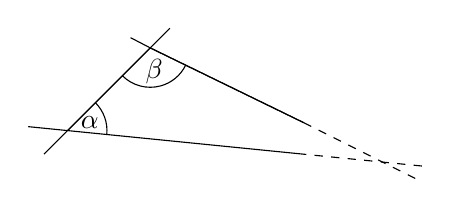
\begin{tikzpicture}
  \draw[dashed]
  (4.5,-0.45)
  -- (3,-0.3) coordinate (a);
  \draw
  (a)
  -- (0,0) coordinate (b) 
  -- (-0.5,0.05)
  (-0.3,-0.3)
  -- (1.3,1.3)
  (0.8,1.18)
  -- (1.05,1.05) coordinate (d) 
  -- (3,0.1) coordinate (e);
  \draw[dashed]
  (e)
  -- (4.5,-0.65);
  \draw
  pic["$\alpha$",draw=black,-,angle eccentricity=0.6,angle radius=0.5cm] {angle=a--b--d};
  \draw
  (b) -- (d) -- (e)
  pic["$\beta$",draw=black,-,angle eccentricity=0.6,angle radius=0.5cm] {angle=b--d--e};
  \end{tikzpicture}
  }
	\caption{Visualisation of the parallel postulate. If the sum of the interior angles $\alpha$ and $\beta$ is less than 180°, the two straight lines, produced indefinitely, meet on that side.}
\end{figure}

Around 1813, Carl Friedrich Gauß worked out that the fifth postulate is in fact independent of the others; that is to say, the parallel postulate as well as its negation can be added to the first four postulates without causing any inconsistencies. While the first case gives us the geometry as postulated by Euclid, the latter revealed a new kind of geometry, commonly referred to as non-Euclidean geometry.

Though Gauß did not publish his finding, it was rediscovered just a few years later. The announcement had a large impact. Suddenly, Euclid's Elements, and with it, the certainty of mathematics, began to totter; in turn, mathematicians became greatly sceptical towards used systems: Which axioms pose the truth? Which will cause harm? Which are dispensable and which are not? Mathematicians sought for confidence in their systems.

What followed in the late 19th century is a series of rigorous axiomatisation of mathematical systems. Giuseppe Peano axiomatised the arithmetic of natural numbers, Moritz Pasch and David Hilbert modernised the foundations of geometry, and Gottlob Frege introduced an axiomatised predicate logic in his revolutionising ``Begriffsschrift'' (German for, roughly, ``concept-script'').

While all these efforts certainly consolidated the trust in given systems, there were some major drawbacks. For one, every system demanded its own foundation and thereby a new set of axioms. Further, albeit it was tried to justify defined axioms, the desire of complete certainty was not met due to the lack of consistency proofs. Thus, it was sought for a consistent-proved, universal system of which all branches of mathematics could then be deduced.

One idea of a universal foundation was given by Georg Cantor around 1880. He introduced a non-formalized kind of set theory, now referred to as naive set theory, in which sets and operations on sets are described with natural language. 

\begin{quote}[Georg Cantor]
``A set is a gathering together into a whole of definite, distinct objects of our perception or of our thought --- which are called elements of the set.''\cite{cantor_set}
\end{quote}

Evidently, such an informal description is not adequate for a study of consistency as it leaves room for ambiguities. Nonetheless, many mathematicians took pleasure in Cantor's set theory and used it as a foundation for different systems.

Frege tried to address the issue of a consistent, universal system in his ``Grundgesetze der Arithmetik'' (German for ``fundamental laws of arithmetic''). He was trying to give a common foundation by reducing all of mathematics, in particular Cantor's set theory, to pure logic, removing all mathematical symbolism. His first efforts had not been well received; however, they still caught the attention of Bertrand Russell. Just as Frege was finishing his final work on his \textit{Grundgesetze}, he received a letter from Russell, which should consequently pose the origin of the foundational crisis. Cantor's set theory as well as Frege's work were casualties of \textit{Russell's paradox} discovered in 1901:
\begin{quote}
Let us consider \textit{the set of all sets that are not members of themselves} denoted by R. In formal notation:
\begin{equation*}
	R\coloneqq\{X\mid X\notin X\}
\end{equation*}
By Cantor's definition, R is indeed a well-defined set.
We are now interested in whether R is a member of itself, that is if $R\in R$ holds.
Let us assume that this is indeed the case. Then, by definition of $R$, it follows that $R$ must not be a member of itself, i.e.\ $R\notin R$, which contradicts our assumption. Now, let us assume the contrary, namely $R\notin R$. Then, again by definition of $R$, we observe that $R$ must be a member of itself, i.e.\ $R\in R$. Hence, we conclude
\begin{equation*}
		R\in R\iff R\notin R
\end{equation*}
which clearly is a contradiction and thus shows the inconsistency of Cantor's set theory.
\end{quote}
Though Frege's work did not contain a definition of sets, it was not difficult for Russell to transfer the paradox to the system constructed by Frege. At the last minute, Frege hastily wrote an appendix for his \textit{Grundgesetze}, in which he explained the issue and proposed a solution by restricting the antinomy-causing axioms of his system; but this was to no avail and consequently caused Frege utter dismay.
\begin{quote}[Gottlob Frege]
``Hardly anything more unfortunate can befall a scientific writer than to have one of the foundations of his edifice shaken after the work is finished. This was the position I was placed in by a letter of Mr. Bertrand Russell, just when the printing of this volume was nearing its completion.''\cite{frege_appendix}
\end{quote}
It was beyond all doubt that Frege's undertaking was dismissed and, even more shocking, the widely established foundation of mathematics, Cantor's naive set theory, was shattered; mathematics was broken at its core. A new, consistent foundation had to be found; a Herculean task, as it turned out, which was tackled by three different schools of thought which we shall discuss next.

\subsection{Logicism --- a foundation made of logic}\label{ssec_logicism}
Mathematics as an extension of logic; this is the central idea of logicism. Although Frege backed up from his endeavours, his pursued idea, the reduction of mathematics to pure logic, was subsequently revisited from Russell and Alfred Whitehead in their famous three-volume work ``Principia Mathematica'' published in 1910--1913.

After the discovery of his paradox, Russell began to study the causes that lead to those kind of antinomies\footnote{There were found antinomies similar to Russel's at the same time, which we are not going to discuss (such as the Burali-Forti paradox or Richard's paradox).\cite{russell_self_referentiality}}. This was an important task because Russell needed to protect his future work from the same bitter fate as experienced by Frege. He concluded that ``in all the contradictions there is a common characteristic, which we may describe as self-reference or reflexiveness''\cite[p. 224]{russell_self_referentiality}. As a means of defence, he invented the idea of type theories. 

In general, a type theory is an extension of a formal system which assigns every object a type. Operations on objects can then be restricted in dependence on involved types.\footnote{For instance, in type-safe programming languages, such as Standard ML or Java, it is not permitted to compare values of different types (e.g.\ integers and strings).} In simple terms, the type theory in Principia Mathematica uses natural numbers as types. A set of type $n$ is then only allowed to contain members of types at most $n-1$. Naturally, this system is not susceptible to antinomies like Russell's as it completely eliminates self-referentiality. 

But Russell recognised that his type theory caused major limitations which made the logical system incapable of representing all of mathematics. In addition, Russell's and Whitehead's attempts in proving the existence of an infinitude of objects using their logical framework failed. Thus, they decided to patch up their system by introducing the \textit{axiom of reducibility} and the \textit{axiom of infinity}; however, these two axioms arguably do not fit the bill.

The former overcomes the limitations caused by Russell's type theory in a fairly specific and technical way. As a result, it was widely criticised that the axiom is too ad hoc and stipulated just in order to attain a desired result.
The latter axiom, on the other hand, guarantees the existence of an infinite amount of objects; but what makes this a logical necessity? Is the universe infinite? Is there an infinite number of atoms?

While Russell's and Whitehead's general intention had been widely advocated, Principia Mathematica was exposed to ever-growing criticisms due to mentioned axioms. They do not seem to be logically self-evident and hence contradict with logicism's central idea. Furthermore, albeit posing a perfection of coherency and precision, the books were known as being illegible due to extremely fine-grained, incremental definitions and rather unusual syntactical notations. They have been described as ``the outstanding example of an unreadable masterpiece.''\cite[p.~154]{math_experience}

\begin{figure}[h]
	\centering
	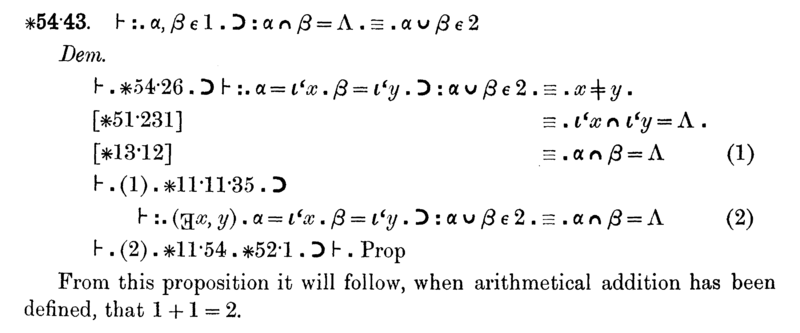
\includegraphics[width=0.8\textwidth]{img/principia_mathematica.png}
	\caption{Principia Mathematica's infamous proof of $1+1=2$. It was not until page 379 that this proof was possible.}
\end{figure}

Nonetheless, the criticisms did not completely debase Russell's and Whitehead's work, but many adopted it as a new mathematical foundation up to 1931 --- the time Gödel once and for all invalidated Russell's and Whitehead's intentions. Yet others were fairly dissatisfied. Among them were the advocates of intuitionism who we shall discuss next.

\subsection{Intuitionism --- proofs with real evidence}\label{ssec_intuitionism}
As opposed to logicism, intuitionism rejects the idea of a mathematics that is completely reducible to some formal system. Intuitionists do not believe that mathematics is existent in a world independent of mankind, but rather it is regarded as the result of constructive mental activities of humans and thereby only existent in humans' minds. In other words, mathematics is based on and conducted by human intuition.

According to Brouwer, the founder of intuitionism, the existence of any mathematical object is equivalent to the possibility of its construction. 
This construction process is neither of a symbolic kind, nor is it reducible to pure logic. Symbols and logic are merely representations used for mental creations. 

This stands in great contrast with classical approaches, in whose the existence of an object can also be proved by refuting its non-existence. As a consequence, intuitionists reject the validity of some assumptions of classical logic, such as the law of excluded middle.
\begin{quote}
\underline{Law of excluded middle:} ``For any proposition P, either P or its negation is true.''\\ 
In logical notation: $\vdash P\lor\lnot P$
\end{quote}
While intuitionistic mathematics is certainly secure from Russell's paradox --- one simply cannot construct such a paradoxical set --- this security comes with a high price as many theorems, in particular those dealing with infinity, rely on laws rejected by intuitionists. For example, let us consider the proof of the following proposition:
\begin{quote}
\textbf{Proposition:} There exist two irrational numbers $a$ and $b$ such that $a^b$ is rational.
\vspace{-2em}
\begin{proof}
	It is known that $\sqrt{2}$ is irrational. Let us consider the number $\sqrt{2}^{\sqrt{2}}$. If it is rational, our statement is proved. If it is irrational, $(\sqrt{2}^{\sqrt{2}})^{\sqrt{2}}=2$ proves our statement.
\end{proof}
\end{quote}
This proof relies on the statement ``either $\sqrt{2}^{\sqrt{2}}$ is rational or it is irrational'' --- an instance of the law of excluded middle --- thus, it is non-constructive and rejected by intuitionists, which seek for more clarity by proving that $\sqrt{2}^{\sqrt{2}}$ is in fact rational (or irrational). Complications like these are the reason the number of scholars who adhere to intuitionism has been staying fairly small.

\begin{quote}[David Hilbert]
``Taking this Tertium non datur (law of excluded middle) from the mathematician would be the same as, say, denying the astronomer his telescope and the boxer the use of his fists.''\cite{hilbert_tertium_non_datur}
\end{quote}

\subsection{Formalism --- mathematics as a symbol modifier}\label{ssec_formalism}
In contrast to logicists and intuitionists, formalists strongly support the autonomy of mathematics. 
They believe that mathematics should be solely based on symbols and axioms that describe syntactical operations on them. Mathematics does not need to justify the existence of its objects, as its objects are just shapes free of any meaning unless they are given an interpretation, which, however, is not part of mathematics according to formalists.

Spearheaded by Hilbert, formalism began to flourish during the period of rigorous axiomatisation in the late 19th century (see section~\ref{ssec_causes}). 
In 1900, Hilbert listed the proof of the consistency of the axioms of arithmetic in his famous \textit{Hilbert's problems}: a list of 23 unsolved fundamental questions which mathematicians should attack during the coming century. As Hilbert was one of the most renowned mathematicians of given time, this was a driving force behind the study of axiom systems.

One of his fellows was Ernst Zermelo. In 1908, Zermelo published his axiomatic set theory on which he had worked for three years. It was supposed to solve the problems of Cantor's naive set theory that had arisen by Russell's paradox, but Zermelo was not able to proof the consistency of his system and stated that the proof is a distant prospect. This arguably was one of the reasons his work was not accepted as a foundation of mathematics up to 1922 when Adolf Fraenkel and Thoralf Skolem independently improved Zermelo's axiom system. 

This new, improved axiom system, known as \textit{Zermelo-Fraenkel set theory}, was eventually able to replace the logical system derived in Principia Mathematica and still poses the foundations of mathematics. Using modern mathematical notation, some of the nine axioms can be formulated as follows:
\small
\begin{enumerate}
    \item \textbf{Axiom of regularity:} Every non-empty set $X$ contains a member $y$ such that $X$ and $y$ are disjoint.
\begin{equation*}
\forall X [\exists a ( a \in X) \rightarrow \exists y ( y \in X \land \lnot \exists z (z \in y \land z \in X))]
\end{equation*}
In particular, this implies that no set is an element of itself.
    \item \textbf{Axiom of specification:} For every predicate $P(\cdot)$ and every set $A$ there exists a set $B$ containing only the elements of $A$ satisfying $P$.
\begin{equation*}
\forall A\,\exists B\,\forall x[x\in B \leftrightarrow \bigl(x\in A \land P(x)\bigr)]
\end{equation*}
This allows us to write $B=\{x\in A\mid P(x)\}$. Further, it can be used to prove the existence of the empty set using some existing set A:
\begin{equation*}
\emptyset\coloneqq\{z\in A\mid (z\in z)\land(z\notin z)\}
\end{equation*}
In fact, the axiom of scheme is an \textit{axiom schema}, that is an infinite series of axioms, since for every predicate $P(\cdot)$ we get a different statement.
    \item \textbf{Axiom of infinity:} There exists an inductive set $X$ (having infinitely many members).
\begin{equation*}
\exists X \left [\emptyset \in X \land \forall y (y \in X \rightarrow y\cup\{y\}  \in X)\right]
\end{equation*}
Note that the axiom has not been exposed to the same extend of criticism as the same-named axiom of Principia Mathematica (see section~\ref{ssec_logicism}), for formalists do not have to justify the meaning of their axioms as they are of a pure syntactic nature.
    \item \textbf{Axiom of choice:} For any set $X$ of nonempty sets, there exists a choice function $f$ defined on $X$. 
\begin{equation*}
\forall X \left[ \emptyset \notin X \rightarrow \exists f\,\forall A(A\in X\rightarrow f(A) \in A ) \right]
\end{equation*}
This axiom is the root of many seemingly paradoxic results, such as the Banach–Tarski paradox, and it was proven being logically independent of the other eight axioms. Nevertheless, it has been accepted by most mathematicians as it is an integral part of many important theorems (e.g.\ every vector space has a basis).
\end{enumerate}
\normalsize
We want to stress that formalists in principle do not assign any fixed semantics to their axioms. The meanings of the axioms (as above) are just given for a better understanding.

Hilbert himself did not focus in finding a new mathematical foundation until 1921 when Hermann Weyl, a former student of Hilbert and formalist, published his paper ``Über die neue Grundlagenkrise der Mathematik'' (German for ``about mathematic's new foundational crisis''). In his paper, Weyl greatly sympathised with Luitzen Brouwer's ideas of intuitionistic mathematics and, to Hilbert's surprise, criticised the pursuit of complete formalisation. Hilbert was dismayed by Weyl's sudden change of stance. He called the intuitionistic idea a ``coup attempt'' which would mitigate mathematics and threaten its most valuable treasures, such as the foundations of set theory.\cite{hilbert_coup}
\begin{quote}[David Hilbert]
``No one shall expel us from the paradise that Cantor has created.''\cite{hilbert_paradise}
\end{quote}
Consequently, Hilbert initiated a research programme called \textit{Hilbert's program} in order to defend his formalistic approach of mathematics. He proposed to clarify the foundations of mathematics using a two-step process: first, a formal system has to be constructed from whose axioms all of mathematics can be derived purely syntactically. The system must only use its axioms, which describe permitted syntactic operations. In particular, the system needs to contain rules for logical terms and deduction rules. This complete formalisation goes beyond the kind of formalisation as provided in former formal axiomatisations, which are satisfied with a listing of assumptions of their specific area of interest. Thereby, mathematics becomes a purely mechanical process whose proofs can be verified by an algorithm.

In the second step, it has to be shown that given axioms never lead to formal inconsistency, e.g.\ that there would exist a proof to derive the term ``$0=1$''. This validation needs to be carried out outside the system using a metamathematical proof. Hilbert proposed that this proof must be of such an elementary character that no one could doubt its soundness, and thus even intuitionistics must accept it. However, neither Hilbert nor anyone else was able to fulfil this wish; not because of a lack of ingenuity, but as it turned out to be unattainable.


\subsection{The peak and the end of the crisis}\label{ssec_end_crisis}
The years after Weyl's change of sides and the consequent initiation of Hilbert's program were characterised by many articles which spread the dispute between the formalistic and intuitionistic schools of thought. On the one hand, intuitionism was criticised being hard to define because its ideas and foundations had been distributed across many papers from Brouwer written only in dutch. On the other hand, Hilbert's program was not fully developed yet but still under construction.

Many mathematicians, however, agreed with Hilbert's warning of the far-reaching limitations of intuitionistic logic. Together with Hilbert's popularity, this caused many scholars to join Hilbert's program. His prolific fellows achieved many important results, notably the proof of consistency of the law of excluded middle by Wilhelm Ackermann in 1925, which largely strengthened confidence in formalism.

The peak of the foundational crisis was reached in 1928. Brouwer boycotted the International Congress of Mathematicians because he solidarised with German mathematicians, whose right of co-determination was dismissed as a result of the first world war. Nevertheless, most Germans still attended the congress, including Hilbert. He consequently was able to present his programme without Brouwer being able to discredit his ideas.

A few days after, Hilbert as one of the major publishers of the prestigious mathematical magazine ``Mathematischen Annalen'' decided to exclude Brouwer as a co-publisher without conducting a referendum. This led to confusion and fierce disputes, but in the end Hilbert's wish came true and Brouwer was expelled. Brouwer, in a state of frustration and despair, subsequently stopped publishing articles concerning his intuitionistic ideas; as a result, intuitionism lost its public attention.  

On the other hand, optimism for a complete and consistent formal foundation of mathematics rose; nonetheless, it was surprisingly crushed in 1931 by Gödel's incompleteness theorems.

\begin{quote}
\underline{First Incompleteness Theorem:} Any consistent formal system F rich enough to contain a formalisation of recursive arithmetic is incomplete, i.e.\ there are statements of the language of F which can neither be proved nor disproved in F.

\underline{Second Incompleteness Theorem:} Any consistent formal system F rich enough to contain a formalisation of recursive arithmetic cannot prove its own consistency.\footnote{These theorems are the improved versions by John Barkley Rosser. Gödel's original theorems were slightly weaker in that they only applied to $\omega$-consistent systems.\cite[pp.~293--320]{fraenkel_incompleteness}}
\end{quote}

These theorems show us that there cannot exist a consistent and complete formal system which is able to prove all of mathematics; hence, they shatter Hilbert's dream and ultimately end the foundational crisis. Ironically, the proof of the theorems is based on self-referentiality within formal systems; something that Hilbert tried to avoid by depriving semantics from mathematics.
We want to give a short sketch of a proof for the first theorem:
\begin{quote}
Let F be a formal system. It is possible to assign every symbol and statement of F a unique number (called Gödel number). For example, let $\Sigma=\{\top,\bot,p,\vtick,\land,\lor,\lnot,(,)\}$ be the alphabet of a formal system for propositional logic in which every variable is of the form $p\vtick^{\ldots}\vtick$, i.e.\ $p,p\vtick,p\vtick\vtick,\ldots$ are variables of the system. We can assign each symbol a unique number using the following mapping:

\begin{center}
\begin{tabular}{| c | c | c | c | c | c | c | c | c |}
\hline $\top$ & $\bot$ & $p$ & \vtick & $\land$ & $\lor$ & $\lnot$ & $($ & $)$ \\
\hline 1 & 2 & 3 & 4 & 5 & 6 & 7 & 8 & 9\\
\hline
\end{tabular}
\end{center}
	For instance, the unique Gödel number of the statement $(p\land p\vtick)\lor \top$ would then be $83534961$. Naturally, if our alphabet contains more than ten symbols, we consequently run out of digits for our mapping. Nevertheless, using the unique prime factorisation of natural numbers, such a numbering is always possible (regardless of the alphabet's size), as shown by Gödel.\cite{goedel_incompleteness}

We can then derive a formula within the system that says ``The statement with Gödel number $x$ is not provable''. Using a diagonalisation argument, we can show that there is a substitution $n$ for $x$ such that the statement with number $n$ translates to ``The statement with Gödel number $n$ is not provable''; in other words, $n$ states ``I am not provable''. We now want to decide whether n is provable in F.

Assume the statement $n$ is provable in F. As $n$ asserts that $n$ is not provable and F is assumed to be sufficiently strong, the negation of $n$ must also be provable, leading to a contradiction.

Now assume the negation of $n$ is provable in F. As F is assumed to be consistent, there must be no Gödel number $m$ that proves $n$ in F. But the negation of $n$ is stating that there is indeed a proof for $n$; thus, F asserts both the non-existence of a proof for n a well as the existence of such a proof.
\end{quote}

\section{Aftermath and prospects}
In 1936, Alonzo Church and Alan Turing independently proved the existence of uncomputable functions and the impossibility of a general solution for Hilbert's \textit{Entscheidungspro\-blem}\footnote{The problem asks for an algorithm that decides whether an input is a valid first-order formula or not.} (German for ``decision problem'') in a similar way as Gödel proved his incompleteness theorems. This shows us that the foundations of computability theory are restricted in the same fashion as the foundations of mathematics and thus sets the limits of computer systems.

Despite Gödel's incompleteness theorems, Hilbert's program was a big success: formalism to this day poses the foundation of modern mathematics, in particular the Zermelo-Fraenkel set theory whose consistency is undoubted by most contemporary mathematicians.  
Formalists do not longer worry about the foundations of mathematics but rather are interested in questions like ``Which axioms do I need at least in order to proof this certain theorem?''. The justification of the axioms itself is regarded philosophical work and is usually not regarded by mathematicians. In fact, most modern mathematicians do not even deal with the foundations of mathematics anymore; instead, they are getting more and more specialised in one single branch of mathematics in order to extend its limits.

While the last few decades have been comparatively free of controversies, we are currently part of the ongoing digitalisation of mathematics; thus, it seems that mathematics will prospectively form an inextricable symbiosis with computer science. Yet proofs and calculations by computers are either regarded an inevitable enrichment or faced with large distrust by mathematicians. It remains to be seen if both parties will be able to concur, or if we shall witness the next controversy of mathematics.

\newpage
\bibliographystyle{plain}
\bibliography{sources.bib}
\end{document}
